\documentclass[11pt]{article}
\usepackage{geometry}                % See geometry.pdf to learn the layout options. There are lots.
\geometry{letterpaper}                   % ... or a4paper or a5paper or ... 
%\geometry{landscape}                % Activate for for rotated page geometry
%\usepackage[parfill]{parskip}    % Activate to begin paragraphs with an empty line rather than an indent
\usepackage[pdftex]{graphicx}
\usepackage{amssymb}
\usepackage{epstopdf}
%\DeclareGraphicsRule{.tif}{png}{.png}{`convert #1 `dirname #1`/`basename #1 .tif`.png}

\newcommand{\Enso}{Ens\={o}}

\title{
\includegraphics[scale=0.15]{enso.png}\\\Enso}
\author{William R. Cook and Tijs van der Storm}
%\date{}                                           % Activate to display a given date or no date

\begin{document}
\maketitle
%\section{}
%\subsection{}


\Enso\ is a theoretically sound and practical reformulation of the 
concepts of model-driven software development. \Enso\ is based
on first-class \textit{structural descriptions}, 
bi-directional \textit{transformations}, \textit{generic operations} 
and \textit{interpretation}.

Structures in \Enso\ are a specialized kind of graph,
whose nodes are either primitive values or collections of observable
properties, whose values are either nodes or collections of nodes.
From a programming language viewpoint this may seem an odd 
choice for data representation. However, it is essentially the
Entity-Relationship (ER) model \cite{FOO}, also known as Information
Models \cite{FOO}, which is widely used in the design of relational databases
and is also the basis for Class Diagrams in 
the Unified Modeling Language (UML) \cite{FOO}, which 
describe the structure of networks of objects.
The key point is that structures in \Enso\ are 
viewed holistically as \textit{graphs}, not as individual values
or traditional sums-and-products data structures.

A structural description, or \textit{schema}, specifies some 
of the observable properties of structures. Schemas are used to
check the consistency structures. Some properties can be checked
while the structure is being created, but other can only be checked
once the structure is complete. \Enso\ allows modification of structures,
which is necessary to create cyclic graphs, but also allows 
valid structures to be sealed to prevent further changes.

Bi-directional transformations are used to map one structure into
another kind of structure, such that mapping can be inverted to 
(partially) recover the original structure from the result.
One common kind of transformation is called a \textit{grammar},
which is a bi-directional transformation between structures and text.
Text grammars are bi-directional because they can be used for parsing
and also rendering. Other transformations include Diagram grammars,
which map structures into diagrams, were edits on the diagram are
reflected in the original structure. GUI grammars are similar.
Transformations are also used for querying, template processing, 
and serialization.

\Enso\ is based on interpretation rather than code generation. 
While it is possible to define transformations that generate code
in conventional languages, this is rarely (if ever) done in \Enso.
Instead all structural descriptions and transformations are 
interpreted dynamically. Although the current incarnation of \Enso\
does not include it, we have previously demonstrated that partial
evaluation can be applied to \Enso-style interpreters to automatically
generate efficient code.

Modularity, generic operations, change management, dynamic creation
of schemas and transformations.
Schemas and transformations are also structures.

What follows is a rapid introduction to the concepts and use of
\Enso. To avoid too many digressions, 
the many connections between \Enso\ and existing approaches,
including programming models
(model-driven, object-oriented, polytypic, functional, constraint-based), theory (dependent types, coalgebra, category theory),
and related ideas (relational databases, domain-specific languages)
are discussed in Section~\ref{relatedwork}.



\subsection{Data}

\Enso\ represents all data via graphs whose structure is defined
by a form of entity-relationship model, called a \textit{schema}. 
\Enso\ shifts focus away from individual pieces of data, to focus instead
on semantically integrated collections of data. 

An \Enso\ data structure is analogous to an information model,
a relational database, an object model without methods, or a coalgebra.
While it is easy to create specialized data modeling notations
in \Enso, the standard information model has the following properties:

Structure are created by \textit{factories}, which create
and manage the nodes in the structure. The factory also
ensures that structures are distinct: a factory identifies the 
collection of nodes that belong to a graph, and any given node 
can only be connected to other nodes in the same graph, which were
created by the same factory.

In \Enso\ most properties of a structure are
checked when the structure is being created. In other words, 
the \textit{factory} that creates the structure is parameterized by a
schema, which the factory uses to check the legality of operations
on the objects it creates.

\subsection{Presentation}






as cyclic graphs, where
nodes are categories into types that have 
consistent attributes and edges are labeled.

All data is represented as cyclic graphs of 


"information model": 
"relational database": the nodes of the graph are
rows of the tables. Foreign keys 

Data is represented as 



This example converts schemas into constructor grammars
\begin{verbatim}
grammar NAME:sym
   CLASSES:
     rule NAME:sym = 
        (SUBTYPES: { NAME:sym "|") "|" @"!SUBTYPES.empty?")?
         [NAME:sym] NAME:str "{" 
            FIELDS: { (NAME:str ":" (NAME:sym): (
                 "[" { TYPE.NAME:sym^ "," } "]"   @"MANY=true"
               | TYPE.NAME:sym^ ?                  @"OPTIONAL=true"
               | TYPE.NAME:sym^
               )) ";" }
             "}"
\end{verbatim}

\subsection{Relationship to Other Approaches}
\label{relatedwork}

\Enso\ data is based on traditional 
entity-relationship (ER) models \cite{FOO},
which are also known as information models. 
ER models were the basis for class diagrams in UML.

In contrast to
object-oriented programming, \Enso\ is focused on holistic
object graphs, rather than individual objects. \Enso\ 
does allow data to include some behavior, for example constraints
and computed fields, but \Enso\ does not associated methods
with data objects.

In contrast to
most theories of functional programming, \Enso\ is based on
coalgebraic signatures rather than algebraic ones. In practice
this means that \Enso\ structures are cyclic graphs rather than
trees. Lazy functional languages can also represent cyclic 
structures, but the cycles are not observable.

\Enso\ supports controlled imperative effects. Objects are
mutable during construction or modification, while the data may be in an
inconstent state, but before it can be used it must be validated
and locked from further changes. This is similar to a transaction.



\section{Requirements for a programming language}

The programming model is based on cyclic graphs.
Graphs are kept distinct from each other. That is,
each graph is considered a self-contained
artifact, without links or pointers to other graphs.

A natural way to create such graphs is with 
imperative effects.

This potentially requires more copying of data
than would be the case in tree-based representations.

To modify graphs, place-holder objects are useful,
as is the ability to "become" another object.

\subsection{Simple reflection}

Fields can be created dynamically and accessed with
"." notation or reflective access.

\begin{verbatim}
o.foo   == o.get("foo")
\end{verbatim}

Assignment to fields can be overriden
\begin{verbatim}
   o.bar = 3   ==> o.set("bar", 3)
\end{verbatim}



\section{QuadModel}

\section{Todos}

* merging schemas and grammars. Need a merge operation. Based on identification/unification

* Finalize on objects, that checks required fields, seals from changes, run invariants
   
* removing "key" from grammar

* fix pretty printing 

* GUIs

* fixedpoint cyclic map





* checked model-objects (with correct inverses and type checking)
* derivative parsers?
* other kind of parser?
* executable UML?
* graphical editors?
    (does Ruby have graphics binding?)
* database mapping?
* WebDSL mini-language




\begin{figure}[htbp]
\begin{center}
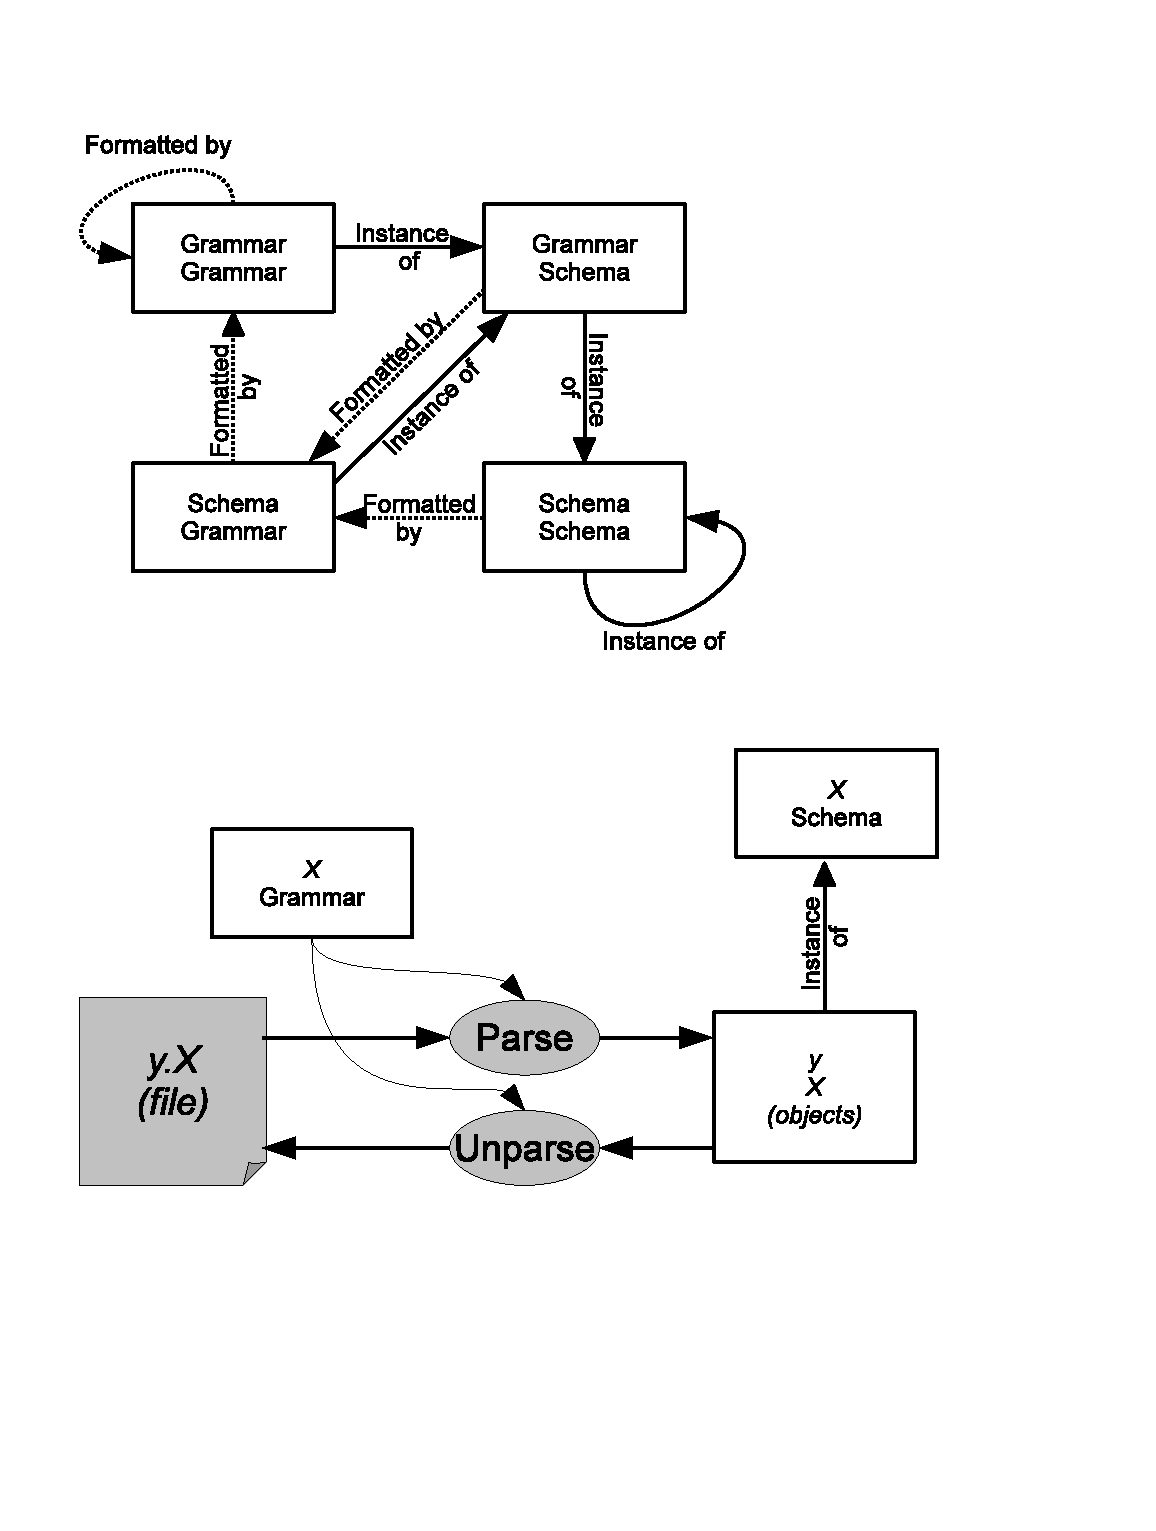
\includegraphics[scale=0.8]{QuadModel.pdf}
\caption{{\bf default}}
\label{default}
\end{center}
\end{figure}



\end{document}  



\begin{itemize}
\item Information models (cyclic graphs) as data structures

\item Types as dynamically checked first-class values

\item Pervasive dynamic creation/transformation of types

\item Generic operations guided by metadata (types, grammars, mappings, etc)

\item Cyclic maps to handle transformation of cyclic structures

\item Uniform handling of textual and visual grammars

\item Fine-grained feature modularity based on mixin composition

\item Pervasive management of change in core, grammars, types, and instances

\item Creation of rich web/GUI/mobile information management applications

\item Dynamic interpretation, code generation only by partial evaluation

\item Bulk operations for efficient remote/database communication

\item Self-implemented, pervasively customizable
\end{itemize}



